\section{Saturnin}
\subsection{Saturnin State structure}

\begin{frame}{Saturnin block and register state}
    \begin{center}
        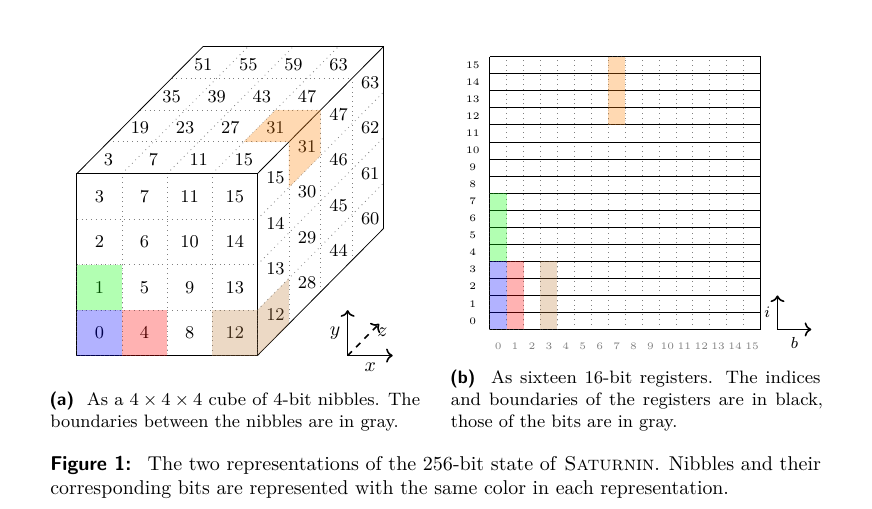
\includegraphics[width=0.85\textwidth,height=0.9\textheight,keepaspectratio]{Images/Figures/1.jpg}
    \end{center}

\end{frame}

\begin{frame}{Terms and Definitions}

\begin{itemize}
    \item Slice: putting the z axis constant
    \item Sheet: putting the x axis constant
    \item Column: putting the x and z as constant
\end{itemize}

\begin{center}
    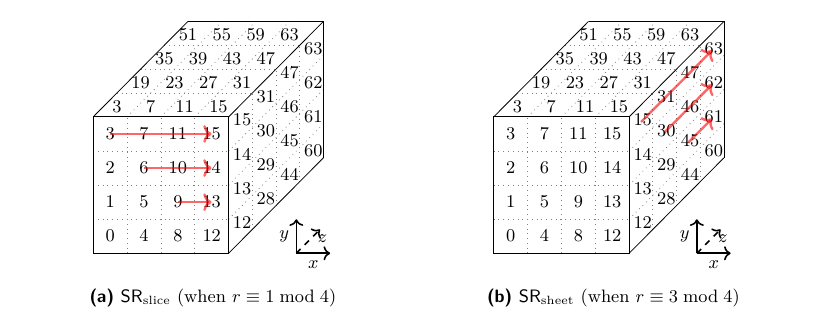
\includegraphics[width=0.85\textwidth,height=0.9\textheight,keepaspectratio]{Images/Figures/2.png}
\end{center}
\end{frame}

\subsection{One round of Saturnin}

\begin{frame}{Sbox}

\begin{center}
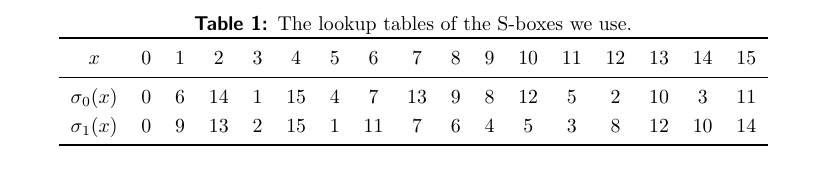
\includegraphics[width=0.9\textwidth,height=0.9\textheight,keepaspectratio]{Images/Figures/sbox.png}
\end{center}

% \begin{itemize}
%     \item SR$_r$ and SR$_r^{-1}$ sandwich the linear layer (MC) for strong diffusion.
%     \item Subkey addition only happens in odd rounds $\rightarrow$ defines a \textbf{super-round}.
% \end{itemize}

\end{frame}

\begin{frame}{Permutation}

    \begin{center}
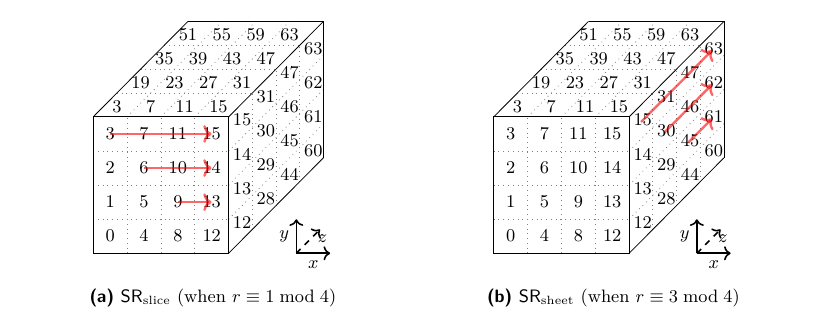
\includegraphics[width=0.9\textwidth,height=0.9\textheight,keepaspectratio]{Images/Figures/2.png}
\end{center}
\end{frame}

\begin{frame}{Permutation}
        \begin{center}
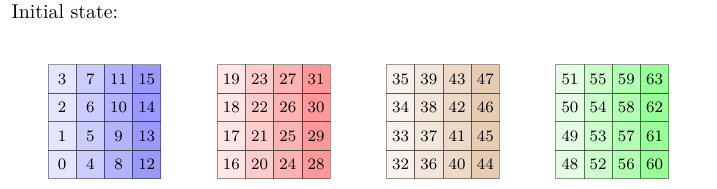
\includegraphics[width=0.9\textwidth,height=0.9\textheight,keepaspectratio]{Images/Figures/p1.png}
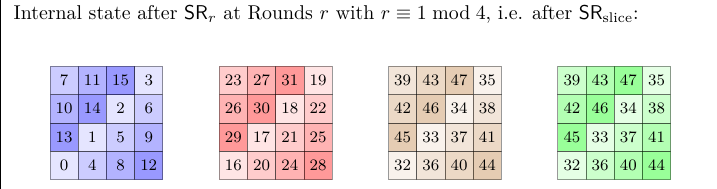
\includegraphics[width=0.9\textwidth,height=0.9\textheight,keepaspectratio]{Images/Figures/p2.png}
\end{center}
\end{frame}

\begin{frame}{Permutation}
        \begin{center}
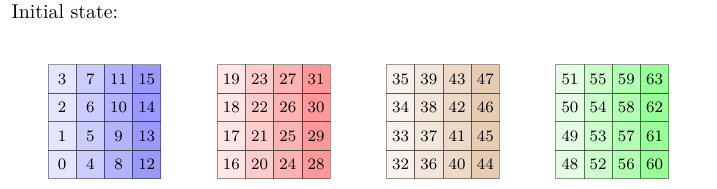
\includegraphics[width=0.9\textwidth,height=0.9\textheight,keepaspectratio]{Images/Figures/p1.png}
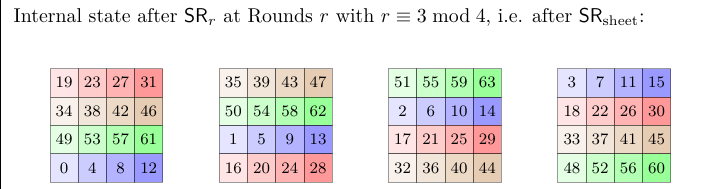
\includegraphics[width=0.9\textwidth,height=0.9\textheight,keepaspectratio]{Images/Figures/p3.png}
\end{center}
\end{frame}

\begin{frame}{Mixed Columns}
            \begin{center}
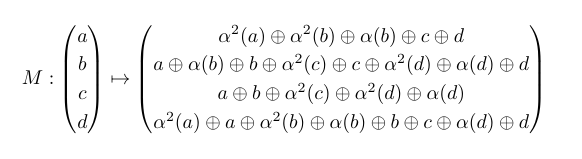
\includegraphics[width=0.7\textwidth,height=0.6\textheight,keepaspectratio]{Images/Figures/mc1.png}
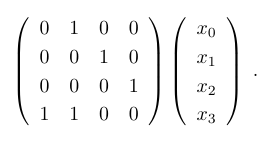
\includegraphics[width=0.45\textwidth,height=0.5\textheight,keepaspectratio]{Images/Figures/mc2.png}
\end{center}
\end{frame}

\begin{frame}{Round function of Saturnin}

\begin{itemize}
    \item One super-round is defined as two round 2r and 2r+1
    \item Each round consists of the following transformations:
    \begin{enumerate}
        \item \textbf{S-box layer (S):} Apply $\sigma_0$ to even-index nibbles and $\sigma_1$ to odd-index nibbles.
        \item \textbf{Permutation (SR$_r$):} 
        \begin{itemize}
            \item Even rounds: Identity
            \item Odd rounds, $r \bmod 4 = 1$: SR$_{\text{slice}}$ (mixes inside slices)
            \item Odd rounds, $r \bmod 4 = 3$: SR$_{\text{sheet}}$ (mixes inside sheets)
        \end{itemize}
        \item \textbf{Linear layer (MC):} Apply 4x4 MDS matrix on each column.
        \item \textbf{Inverse permutation (SR$_r^{-1}$):} Undo the SR$_r$ applied earlier.
        \item \textbf{Subkey addition:} At the end of each super-round (odd rounds), XOR with round key + round constant.
    \end{enumerate}
\end{itemize}

\end{frame}

\section{Security}
\begin{frame}{Saturnin Security}
    \begin{itemize}
        \item Security wise: 1 super round of Saturnin = 1 round of AES
        \item Therefore, the number of rounds is 20 or 2*10(AES)
    \end{itemize}
\end{frame}
